\documentclass[10pt,a4paper]{article}

\usepackage[margin=2.2cm]{geometry}
\usepackage[T1]{fontenc}
\usepackage[utf8]{inputenc}
\usepackage{lmodern}
\usepackage{amsmath,amssymb}
\usepackage{booktabs}
\usepackage{tikz}
\usepackage{array}
\usepackage{enumitem}
\usepackage{graphicx}
\usepackage{microtype}
\usepackage[colorlinks=true,linkcolor=black,citecolor=black,urlcolor=blue]{hyperref}

\setlist{itemsep=1pt, topsep=2pt, parsep=0pt}
\renewcommand{\topfraction}{0.9}
\renewcommand{\bottomfraction}{0.8}
\renewcommand{\textfraction}{0.07}
\renewcommand{\floatpagefraction}{0.75}

\title{LLM-Based Agentic Monitoring vs.\ Classical Change-Point Detection for
Financial Market Regime Identification}
\author{Oscar Pham \& Paul Chen}
\date{\today}

\begin{document}
\maketitle

\begin{abstract}
We present a preregistered experiment comparing an LLM-based agentic monitoring
system to classical change-point detectors for identifying regime breaks in two
quantitative trading strategies. The agentic system integrates a small language
model (qwen2.5:1.5b with grammar-constrained decoding) with filtered financial
news, macroeconomic vintages, and strategy telemetry through a triage-escalation
architecture; the classical arm uses Page-Hinkley, BOCPD, HMM, and
distributional-threshold detectors. Both arms observe identical point-in-time
data across 12 historical windows (2004--2020), split into a development set and
a sequestered confirmatory test set. On the development set (8 event pairs), the
agentic system detects regime breaks 9.75 days earlier on average (exact
permutation $p = 0.0039$, Holm-adjusted $p = 0.0156$) with recall 8/8 versus 6/8
for classical. The test set (5 pairs) is directionally consistent ($-4.4$ days,
$p = 0.25$) but structurally underpowered. The false-positive-rate co-primary
endpoint does not favour the agentic arm. A three-condition leakage harness
bounds pretraining memorisation, and an exploratory PnL simulation suggests the
latency advantage translates to meaningful drawdown reduction. The results
provide suggestive but not confirmatory evidence that multi-signal LLM fusion
reduces detection latency relative to classical statistical methods.
\end{abstract}

% ============================================================
\section{Introduction}\label{sec:intro}

Quantitative trading strategies are subject to regime breaks. The August 2007
quant meltdown (Khandani \& Lo, 2007), the 2009 momentum crash (Daniel \&
Moskowitz, 2016), and the February 2018 volatility event demonstrate that such
breaks can destroy years of accumulated profit within days. Classical
change-point methods, Page-Hinkley (1954), Bayesian online change-point
detection (Adams \& MacKay, 2007), hidden Markov models (Hamilton, 1989), and
threshold rules, operate exclusively on the strategy's return stream and react
only after its statistical properties have already shifted. If news coverage of
a developing crisis precedes its statistical manifestation in returns, an
LLM-based monitor that fuses telemetry with natural-language context might
detect regime breaks earlier.

We report a preregistered experiment testing three hypotheses:
\textbf{H1 (co-primary):} the agentic system achieves both lower detection
latency and lower false-positive rate (FPR) than the best classical detector;
\textbf{H2:} any advantage generalises across both strategies;
\textbf{H3:} the magnitude of advantage differs by strategy.

Our contributions are: (1)~a three-layer agentic monitoring architecture running
a 1.5B-parameter model on consumer hardware; (2)~an evaluation protocol with
strict information parity on a survivorship-bias-free universe, a distinction
that reverses the sign of the anchor event ($+3.4\%$ on a survivor-only universe
against a $-4.8\%$ drawdown point-in-time); (3)~a three-condition leakage
harness separating genuine detection from recall of famous events; and (4)~full
disclosure of protocol deviations and operational failure modes.

% ============================================================
\section{Data and Strategies}\label{sec:data}

All inputs are constructed point-in-time (PIT): on any decision date $t$, both
arms observe only values published on or before $t$. The eligible universe is
reconstructed from historical S\&P~500 constituent membership intervals
(${\sim}347$ eligible names per month, versus ${\sim}542$ under a survivor-only
universe). Two daily PnL series are built on this universe:

\textbf{AL\_PCA} (Avellaneda \& Lee, 2010): sector-sleeve PCA mean reversion
($K = 15$ components; Ornstein--Uhlenbeck residual z-scores with fixed
entry/exit thresholds), spanning 2003--2014.
\textbf{JT\_MOM} (Jegadeesh \& Titman, 1993): cross-sectional momentum (12-1
ranking, long top decile, short bottom decile, monthly rebalance), spanning
2003--2020. Daily return correlation between the two series is ${\sim}0.003$;
this near-orthogonality is what makes the cross-strategy hypotheses informative.
The AL\_PCA curve ends in 2014, excluding it from three of four test-set events
and reducing the confirmatory sample to five pairs (Section~\ref{sec:power}).

News context comes from the FNSPID corpus (Dong et al., 2024): ${\sim}11.8$M
articles (2003--2020) in per-year Parquet files, queried over a 7-day trailing
window with a risk-term filter. Article density is uneven (${\sim}2{,}800$/day
in 2007--2016, ${\sim}80$/day pre-2007, ${\sim}1{,}400$/day 2017--2020); the NYT
Archive API supplements sparse pre-2010 windows. Macroeconomic context uses
ALFRED \emph{vintage} series (first-print values as published on the decision
date) rather than revised FRED series, closing a revision-lookahead channel.

% ============================================================
\section{Method}\label{sec:method}

\subsection{Classical Arm}\label{sec:method-classical}

Four detectors operate on the daily return stream: Page-Hinkley
($\delta = 0.5$, $\lambda = 8.0$), BOCPD (hazard $1/250$), a two-state Gaussian
HMM (low- to high-volatility transition), and a rolling z-score threshold. An
aggregate alarm fires when ${\geq}2$ detectors fire within 5 trading days. For
the primary H1 analysis the best single detector (HMM) is the headline
comparator, since the aggregation rule's latency penalty makes it the weaker
(less conservative) baseline.

\subsection{Agentic Arm}\label{sec:method-agentic}

Each trading day passes through three layers (Figure~\ref{fig:architecture}):
\emph{triage}, a \emph{news context agent}, and a \emph{performance supervisor},
sharing a guardrail module that enforces information parity with the classical
arm.

\begin{figure}[htbp]
\centering
\resizebox{0.92\textwidth}{!}{%
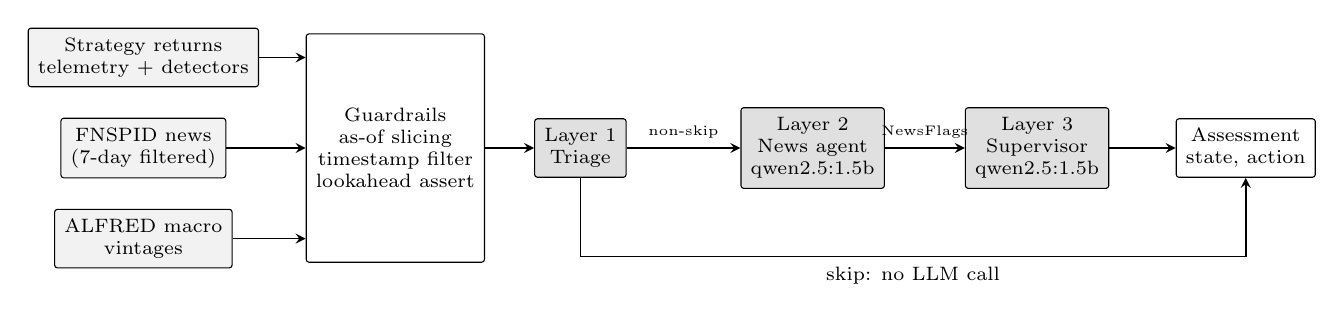
\begin{tikzpicture}[
  font=\scriptsize,
  box/.style={draw, rounded corners=1pt, align=center, inner sep=3.5pt},
  agent/.style={box, fill=black!12},
  arrow/.style={->, >=stealth, semithick}
]
\node[box, fill=black!5] (ret)   at (0, 1.15) {Strategy returns\\telemetry + detectors};
\node[box, fill=black!5] (news)  at (0, 0.0)  {FNSPID news\\(7-day filtered)};
\node[box, fill=black!5] (macro) at (0,-1.15) {ALFRED macro\\vintages};
\node[box, minimum height=2.9cm] (guard) at (3.2, 0)
  {Guardrails\\as-of slicing\\timestamp filter\\lookahead assert};
\node[agent] (triage) at (5.55, 0) {Layer 1\\Triage};
\node[agent] (na)     at (8.5, 0)  {Layer 2\\News agent\\qwen2.5:1.5b};
\node[agent] (sup)    at (11.35, 0){Layer 3\\Supervisor\\qwen2.5:1.5b};
\node[box]   (out)    at (14.0, 0) {Assessment\\state, action};
\draw[arrow] (ret)   -- (guard.west |- ret);
\draw[arrow] (news)  -- (guard);
\draw[arrow] (macro) -- (guard.west |- macro);
\draw[arrow] (guard) -- (triage);
\draw[arrow] (triage) -- node[above, pos=0.5]{\tiny non-skip} (na);
\draw[arrow] (na) -- node[above, pos=0.5]{\tiny NewsFlags} (sup);
\draw[arrow] (sup) -- (out);
\draw[arrow] (triage.south) -- ++(0,-1.0) -| node[pos=0.25, below]{skip: no LLM call} (out.south);
\end{tikzpicture}%
}
\caption{Agentic architecture. All inputs pass through fail-closed guardrails
before the three-layer pipeline; triage routes each day to \textsc{skip} (no
LLM call) or to progressively richer inference modes.}
\label{fig:architecture}
\end{figure}

\textbf{Triage.} Three causal signals set the per-day compute budget: FinBERT
stress $s$ (daily-maximum negative-sentiment probability over filtered
headlines), a trailing-baseline news-intensity $z$-score of risk-term hits, and
the count $n$ of classical detectors alarming within 3 calendar days. The rule
(fixed a priori) is
\[
\text{mode} =
\begin{cases}
\textsc{classical\_escalation} & \text{if } \geq 2 \text{ detectors within 5 days} \\
\textsc{thinking}              & \text{if } s \geq 0.60 \;\lor\; z \geq 2.0 \;\lor\; n \geq 1 \\
\textsc{cheap}                 & \text{if } s \geq 0.30 \\
\textsc{skip}                  & \text{otherwise.}
\end{cases}
\]

\textbf{News context agent.} Non-skip days send up to 40 risk-filtered articles
from the 7-day trailing query to the model, which emits structured
\texttt{NewsFlags} JSON (overall risk level, flagged evidence, narrative,
confidence). Output is grammar-constrained (Ollama \texttt{format=json}); one
repair retry is attempted, and persistent failures are logged and the day
proceeds without news flags.

\textbf{Performance supervisor.} The supervisor receives causally sliced
telemetry (trailing 60-day statistics, drawdown), classical detector alarms,
ALFRED macro context, and the news flags, and emits an assessment with
$\texttt{state} \in \{\text{NORMAL},\text{WATCH},\text{ALERT},\text{CRITICAL}\}$
and an action recommendation. A day is an \emph{alarm} if state
$\in \{\text{ALERT},\text{CRITICAL}\}$; alarm clusters are de-duplicated with a
5-trading-day cooldown.

\textbf{Guardrails.} Four fail-closed checks enforce parity: (1)~as-of slicing
of telemetry and alarms; (2)~a publication-timestamp filter on articles; (3)~a
future-text scrub dropping articles embedding any ISO date past the decision
date; (4)~a recursive lookahead assertion over the full context that raises a
hard error on violation.

\textbf{Model.} Both agents use qwen2.5:1.5b via Ollama at temperature 0. The
preregistered llama3.2:3b was substituted before any evaluation after failing
structured-output benchmarks (11/30 valid JSON vs.\ 30/30; Deviation~1). Full
prompts and schemas are in the repository.

\subsection{Endpoints and Analysis Plan}\label{sec:method-endpoints}

All metrics, tests, and decision rules were fixed before an evaluation freeze
(git tag \texttt{eval-freeze-v1}); no thresholds were tuned on evaluation data.

\textbf{Latency (co-primary).} For each event window with preregistered onset
$t_\text{onset}$, latency is $\ell = t_\text{alarm} - t_\text{onset}$ (calendar
days) for the first alarm in $[t_\text{onset}, t_\text{onset}+21\text{d}]$
(agentic: ALERT/CRITICAL; classical: HMM). Misses are right-censored at
$\ell = 21$ so non-detections enter as worst-case latencies.

\textbf{FPR (co-primary).} During calm windows every alarm is false. Agentic
FPR counts de-duplicated cluster starts per trading day; classical FPR counts
every alarm day. This asymmetry (Deviation~9) biases in favour of the agentic
arm, so a null FPR result is robust a fortiori.

\textbf{Secondary.} Recall (binary detection in the 21-day zone; runtime
failures count as misses) and an onset-sensitivity re-scoring against
curve-derived onsets (peak before deepest trough).

\textbf{Tests.} Latency: exact permutation over all $2^n$ sign-flips of paired
differences (one-sided). FPR: moving-block bootstrap ($b = 10$\,d,
$B = 10{,}000$, seed 42; two-sided), with Fisher's exact as a check. Recall:
McNemar exact and a Beta--Binomial posterior (Jeffreys prior). The two
co-primary $p$-values are Holm-corrected ($k = 2$); H1 is \emph{supported} if
both reject at family-wise $\alpha = 0.05$, \emph{partially supported} if one
rejects. H2 is assessed directionally per strategy; H3 as the interaction
$\Delta_\text{AL\_PCA} - \Delta_\text{JT\_MOM}$.

\textbf{A priori power bound.} With $n$ pairs the permutation test's minimum
$p$ is $2^{-n}$: $1/256$ for the development set ($n = 8$) but $1/32$ for the
test set ($n = 5$), whose Holm-adjusted best case $2/32 = 0.0625$ cannot reject
at $\alpha = 0.05$. The confirmatory set is structurally underpowered, a
limitation acknowledged before unblinding.

\subsection{Evaluation Protocol}\label{sec:protocol}

Twelve windows are split into a development set (events: quant meltdown 2007,
GFC/Lehman 2008, momentum crash 2009, US downgrade 2011; calm: 2004--2006,
2013--2014) and a sequestered test set (events: flash crash 2010, China
devaluation 2015, volmageddon 2018, COVID-19 2020; calm: 2012, 2017). The
partition was fixed before any runs; test windows were accessed only after an
automated freeze gate (11 checks) passed on the tagged codebase. After the tag,
no prompt, threshold, or scoring rule changed; post-freeze infrastructure fixes
(context caching, dead-runner recovery, thermal-stall reruns) affect
availability only and are logged as Deviations 12--15.

To bound pretraining memorisation, a leakage harness runs three conditions:
\textbf{A} (standard), \textbf{B} (all ISO dates replaced by a non-parseable
sentinel, preserving numerical evidence while blocking memorised event--date
associations), and \textbf{C} ($M = 10$ synthetic windows with fabricated news
and shuffled returns). The preregistered bound is
$\text{memorisation} \leq \text{perf}_A - \min(\text{perf}_B, \text{perf}_C)$,
with detection classified evidence-driven if
$\min(\text{perf}_B, \text{perf}_C) \geq 0.6\,\text{perf}_A$.

All experiments ran on one consumer laptop (i7-11800H, 32\,GB RAM, RTX 3050 Ti
4\,GB VRAM; FinBERT on CPU to avoid VRAM contention). Fifteen deviations from
the preregistration are fully documented in \texttt{docs/DEVIATIONS.md} in the
repository; the most consequential are cited inline.

% ============================================================
\section{Results}\label{sec:results}

\subsection{Detection Latency}\label{sec:results-latency}

Table~\ref{tab:latency} reports all paired latencies. On the development set
the agentic system detects 9.75 days earlier on average (exact permutation
$p = 0.0039$; Holm $p = 0.0156$), rejecting $H_0$. The test set is
directionally consistent ($-4.4$ days) but not significant ($p = 0.25$,
$n = 5$).

\begin{table}[htbp]
\centering
\footnotesize
\caption{Paired detection latency (calendar days from onset). ``Cens.''\ marks
non-detections imputed at $\ell = 21$\,d. Classical comparator is HMM.}
\label{tab:latency}
\begin{tabular}{llrrrl}
\toprule
Window & Strategy & Classical & Agentic & $\Delta$ & Set \\
\midrule
Quant meltdown 2007  & AL\_PCA & 7  & 0  & $-7$  & Dev \\
GFC / Lehman 2008    & AL\_PCA & 14 & 0  & $-14$ & Dev \\
Momentum crash 2009  & AL\_PCA & 1  & 0  & $-1$  & Dev \\
Downgrade 2011       & AL\_PCA & 11 & 5  & $-6$  & Dev \\
Quant meltdown 2007  & JT\_MOM & 7  & 0  & $-7$  & Dev \\
GFC / Lehman 2008    & JT\_MOM & Cens. & 2  & $-19$ & Dev \\
Momentum crash 2009  & JT\_MOM & Cens. & 1  & $-20$ & Dev \\
Downgrade 2011       & JT\_MOM & 7  & 3  & $-4$  & Dev \\
\addlinespace
Flash crash 2010     & AL\_PCA & 8  & 5  & $-3$  & Test \\
Flash crash 2010     & JT\_MOM & Cens. & 1  & $-20$ & Test \\
China deval.\ 2015   & JT\_MOM & 2  & 9  & $+7$  & Test \\
Volmageddon 2018     & JT\_MOM & Cens. & 8  & $-13$ & Test \\
COVID-19 2020        & JT\_MOM & 14 & Cens. & $+7$  & Test \\
\midrule
\multicolumn{2}{l}{\emph{Dev mean (8 pairs)}} & 11.1 & 1.38 & $-9.75$ & \\
\multicolumn{2}{l}{\emph{Test mean (5 pairs)}} & 13.2 & 8.8 & $-4.4$ & \\
\bottomrule
\end{tabular}
\end{table}

\begin{figure}[htbp]
\centering
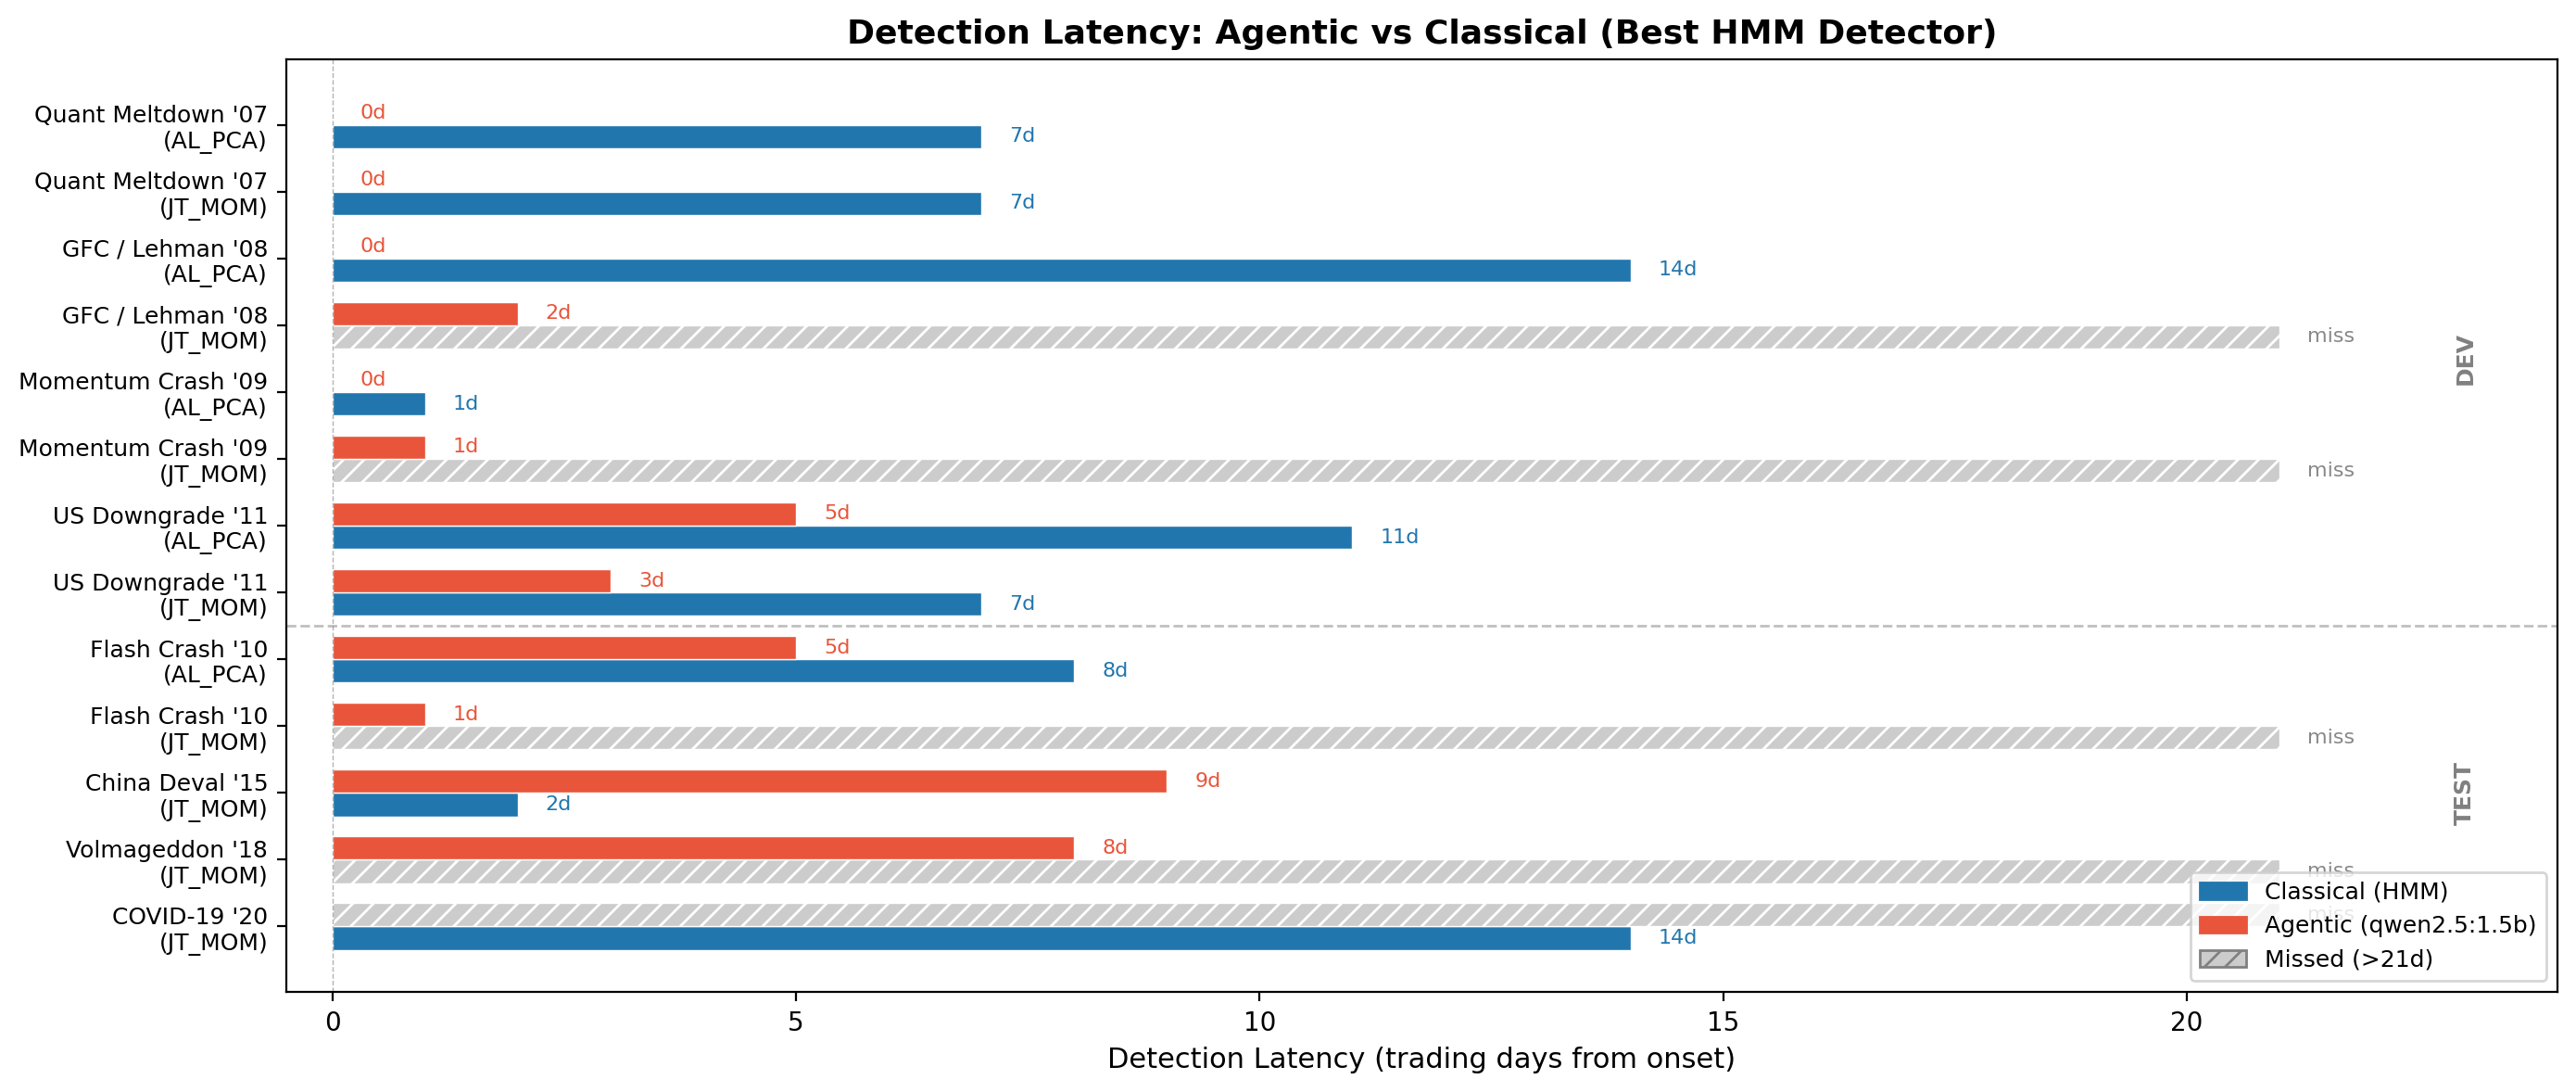
\includegraphics[width=0.78\textwidth]{monitoring/results/figures/fig1_latency_bars.png}
\caption{Detection latency per event window: agentic (red) versus classical
HMM (blue); shorter bars are better. Hatched bars denote misses censored at
21 days.}
\label{fig:latency-bars}
\end{figure}

\subsection{False-Positive Rate}\label{sec:results-fpr}

Table~\ref{tab:fpr} reports per-calm-window FPR. Development-set agentic FPR
(1.31\%) is statistically indistinguishable from classical HMM (1.08\%):
bootstrap $p = 0.62$ (95\% CI for the difference $[-0.42, +0.88]$\,pp), Holm
$p = 0.62$. On the test set the agentic arm is \emph{worse} (6.93\% vs.\
1.41\%, $p = 0.51$), driven by calm 2012. There is no evidence of an agentic
FPR advantage.

\begin{table}[htbp]
\centering
\footnotesize
\caption{False-positive rate per calm window (agentic: alarm cluster starts /
trading days; classical: alarm days / trading days, cf.\ Deviation~9).}
\label{tab:fpr}
\begin{tabular}{llrrl}
\toprule
Calm window & Strategy & Classical & Agentic & Set \\
\midrule
2004--2006   & AL\_PCA & 3.05\% & 0.13\% & Dev \\
2004--2006   & JT\_MOM & 0.53\% & 0.13\% & Dev \\
2013--2014   & AL\_PCA & 0.00\% & 3.84\% & Dev \\
2013--2014   & JT\_MOM & 0.20\% & 2.30\% & Dev \\
\addlinespace
2012         & AL\_PCA & 1.20\% & 10.38\% & Test \\
2012         & JT\_MOM & 2.00\% & 7.69\% & Test \\
2017         & JT\_MOM & 1.20\% & 2.70\% & Test \\
\midrule
\emph{Dev aggregate}  & & 1.08\% & 1.31\% & \\
\emph{Test aggregate} & & 1.41\% & 6.93\% & \\
\bottomrule
\end{tabular}
\end{table}

\begin{figure}[htbp]
\centering
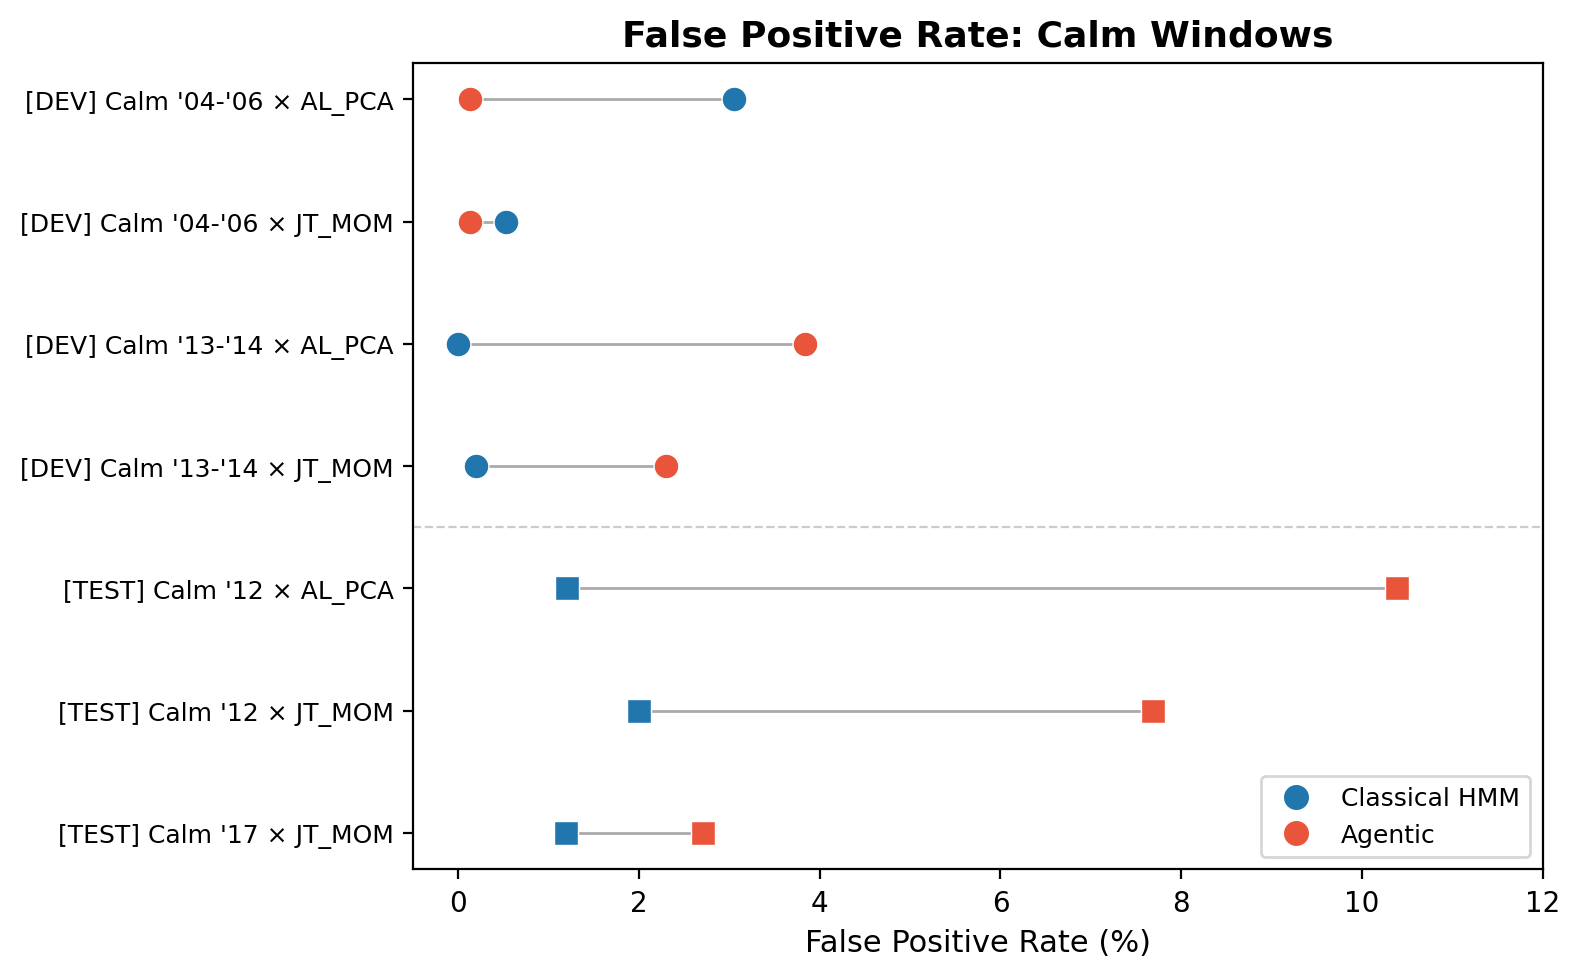
\includegraphics[width=0.62\textwidth]{monitoring/results/figures/fig2_fpr_dotplot.png}
\caption{False-positive rate per calm window. Agentic FPR is comparable on the
development set but elevated on the test set, particularly calm 2012.}
\label{fig:fpr-dot}
\end{figure}

\subsection{Recall and H1 Verdict}\label{sec:results-recall}

Development recall is 8/8 agentic vs.\ 6/8 classical (McNemar $p = 0.50$;
posterior $P(\theta_A > \theta_C) = 0.936$); test recall is 4/5 vs.\ 3/5
(McNemar $p = 1.0$; posterior $0.75$). Applying the preregistered rule, H1 is
\textbf{partially supported}: latency rejects on the development set (Holm
$p = 0.0156$) but FPR does not (Holm $p = 0.62$). On the test set neither
endpoint rejects; the confirmatory analysis is inconclusive for lack of power.

\subsection{Strategy Breakdown (H2, H3)}\label{sec:results-strategy}

The latency advantage is directionally consistent across both strategies on
the development set: AL\_PCA mean $\Delta = -7.0$\,d, JT\_MOM $-12.5$\,d
(both 4 pairs), supporting H2 directionally; on the test set both directions
remain agentic-favourable (AL\_PCA $-3$\,d on 1 pair; JT\_MOM $-4.75$\,d on 4).
The H3 interaction is $+5.5$\,d: JT\_MOM benefits more
(Figure~\ref{fig:strategy}), because the classical HMM missed GFC 2008 and
momentum crash 2009 entirely on momentum returns while news coverage clearly
signalled stress.

\begin{figure}[htbp]
\centering
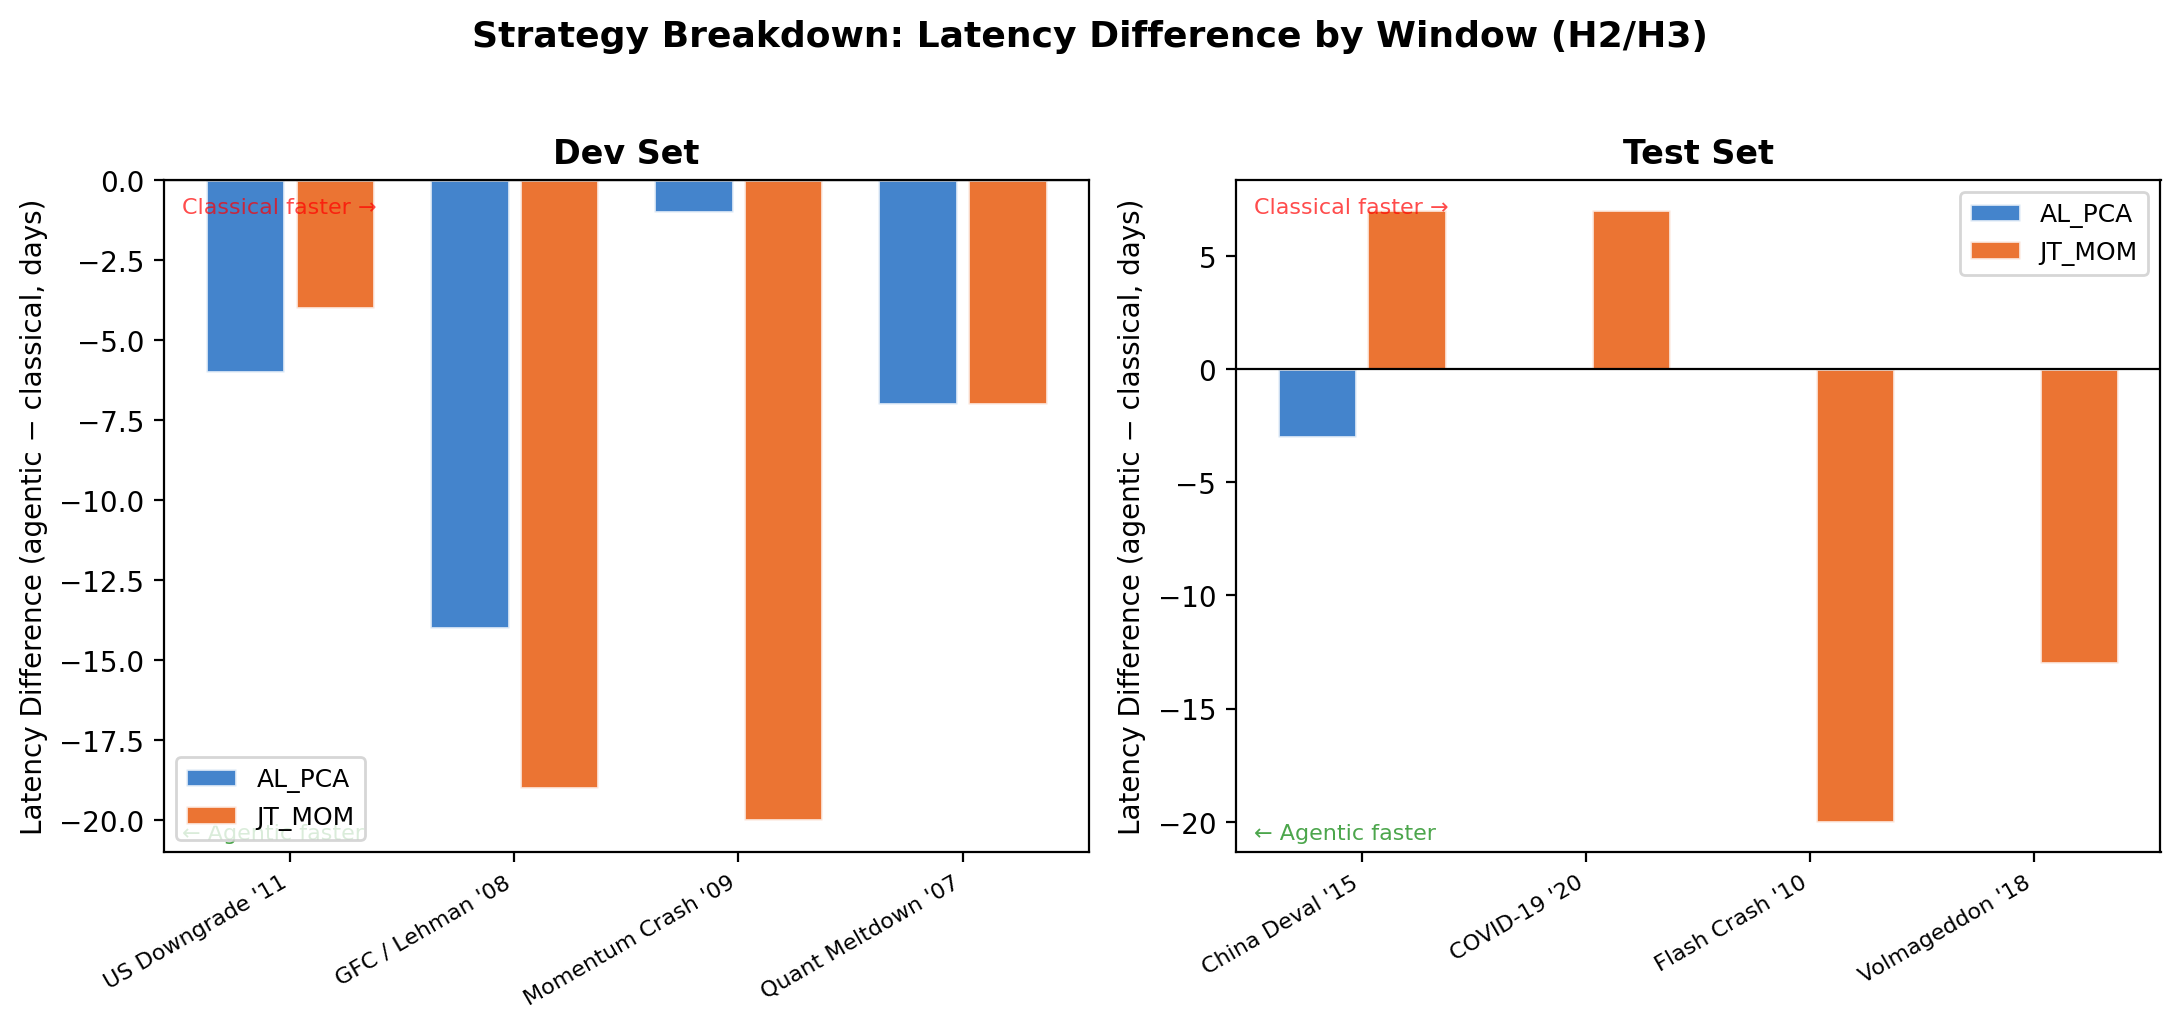
\includegraphics[width=0.68\textwidth]{monitoring/results/figures/fig7_strategy_breakdown.png}
\caption{Per-strategy latency advantage (development set). JT\_MOM benefits
more, primarily because the HMM misses two events on momentum returns.}
\label{fig:strategy}
\end{figure}

\subsection{Economic Significance (Exploratory)}\label{sec:results-pnl}

We simulate three regimes per event window: unmonitored, classical-monitored
(flatten at first HMM alarm), and agentic-monitored (flatten at first ALERT or
CRITICAL), with no transaction costs and no re-entry. Across the 13 event
pairs (Table~\ref{tab:pnl}, Figure~\ref{fig:dd-avoided}), mean maximum
drawdown avoided is 1.82\,pp (classical) versus 10.09\,pp (agentic), an
advantage of 8.28\,pp per event. The extreme case is momentum crash 2009 on
JT\_MOM: the unmonitored strategy lost 94.47\%, the HMM never fired, and the
agentic exit avoided 72.28\,pp. Excluding this window the mean advantage is
2.95\,pp. China devaluation 2015 is the only reversal ($-1.72$\,pp): the
agentic alarm fired 21 July, exiting before a partial recovery, while the
classical alarm on 13 August was better timed. These idealised assumptions
overstate absolute value but affect both arms symmetrically.

\begin{table}[htbp]
\centering
\footnotesize
\caption{Maximum drawdown avoided (pp) relative to the unmonitored baseline.}
\label{tab:pnl}
\begin{tabular}{llrrr}
\toprule
Window & Strategy & Classical & Agentic & Advantage \\
\midrule
Quant meltdown 2007  & AL\_PCA & 3.05 & 6.90 & 3.85 \\
GFC / Lehman 2008    & AL\_PCA & 1.82 & 3.16 & 1.34 \\
Momentum crash 2009  & AL\_PCA & 2.10 & 4.00 & 1.90 \\
Downgrade 2011       & AL\_PCA & 0.00 & 0.06 & 0.06 \\
Quant meltdown 2007  & JT\_MOM & 0.00 & 1.47 & 1.47 \\
GFC / Lehman 2008    & JT\_MOM & 0.00 & 15.63 & 15.63 \\
Momentum crash 2009  & JT\_MOM & 0.00 & 72.28 & 72.28 \\
Downgrade 2011       & JT\_MOM & 4.66 & 7.30 & 2.64 \\
Flash crash 2010     & AL\_PCA & 2.38 & 3.49 & 1.11 \\
Flash crash 2010     & JT\_MOM & 6.15 & 10.34 & 4.19 \\
China deval.\ 2015   & JT\_MOM & 3.44 & 1.72 & $-1.72$ \\
Volmageddon 2018     & JT\_MOM & 0.00 & 0.00 & 0.00 \\
COVID-19 2020        & JT\_MOM & 0.00 & 4.87 & 4.87 \\
\midrule
\emph{Mean} & & 1.82 & 10.09 & 8.28 \\
\bottomrule
\end{tabular}
\end{table}

\begin{figure}[htbp]
\centering
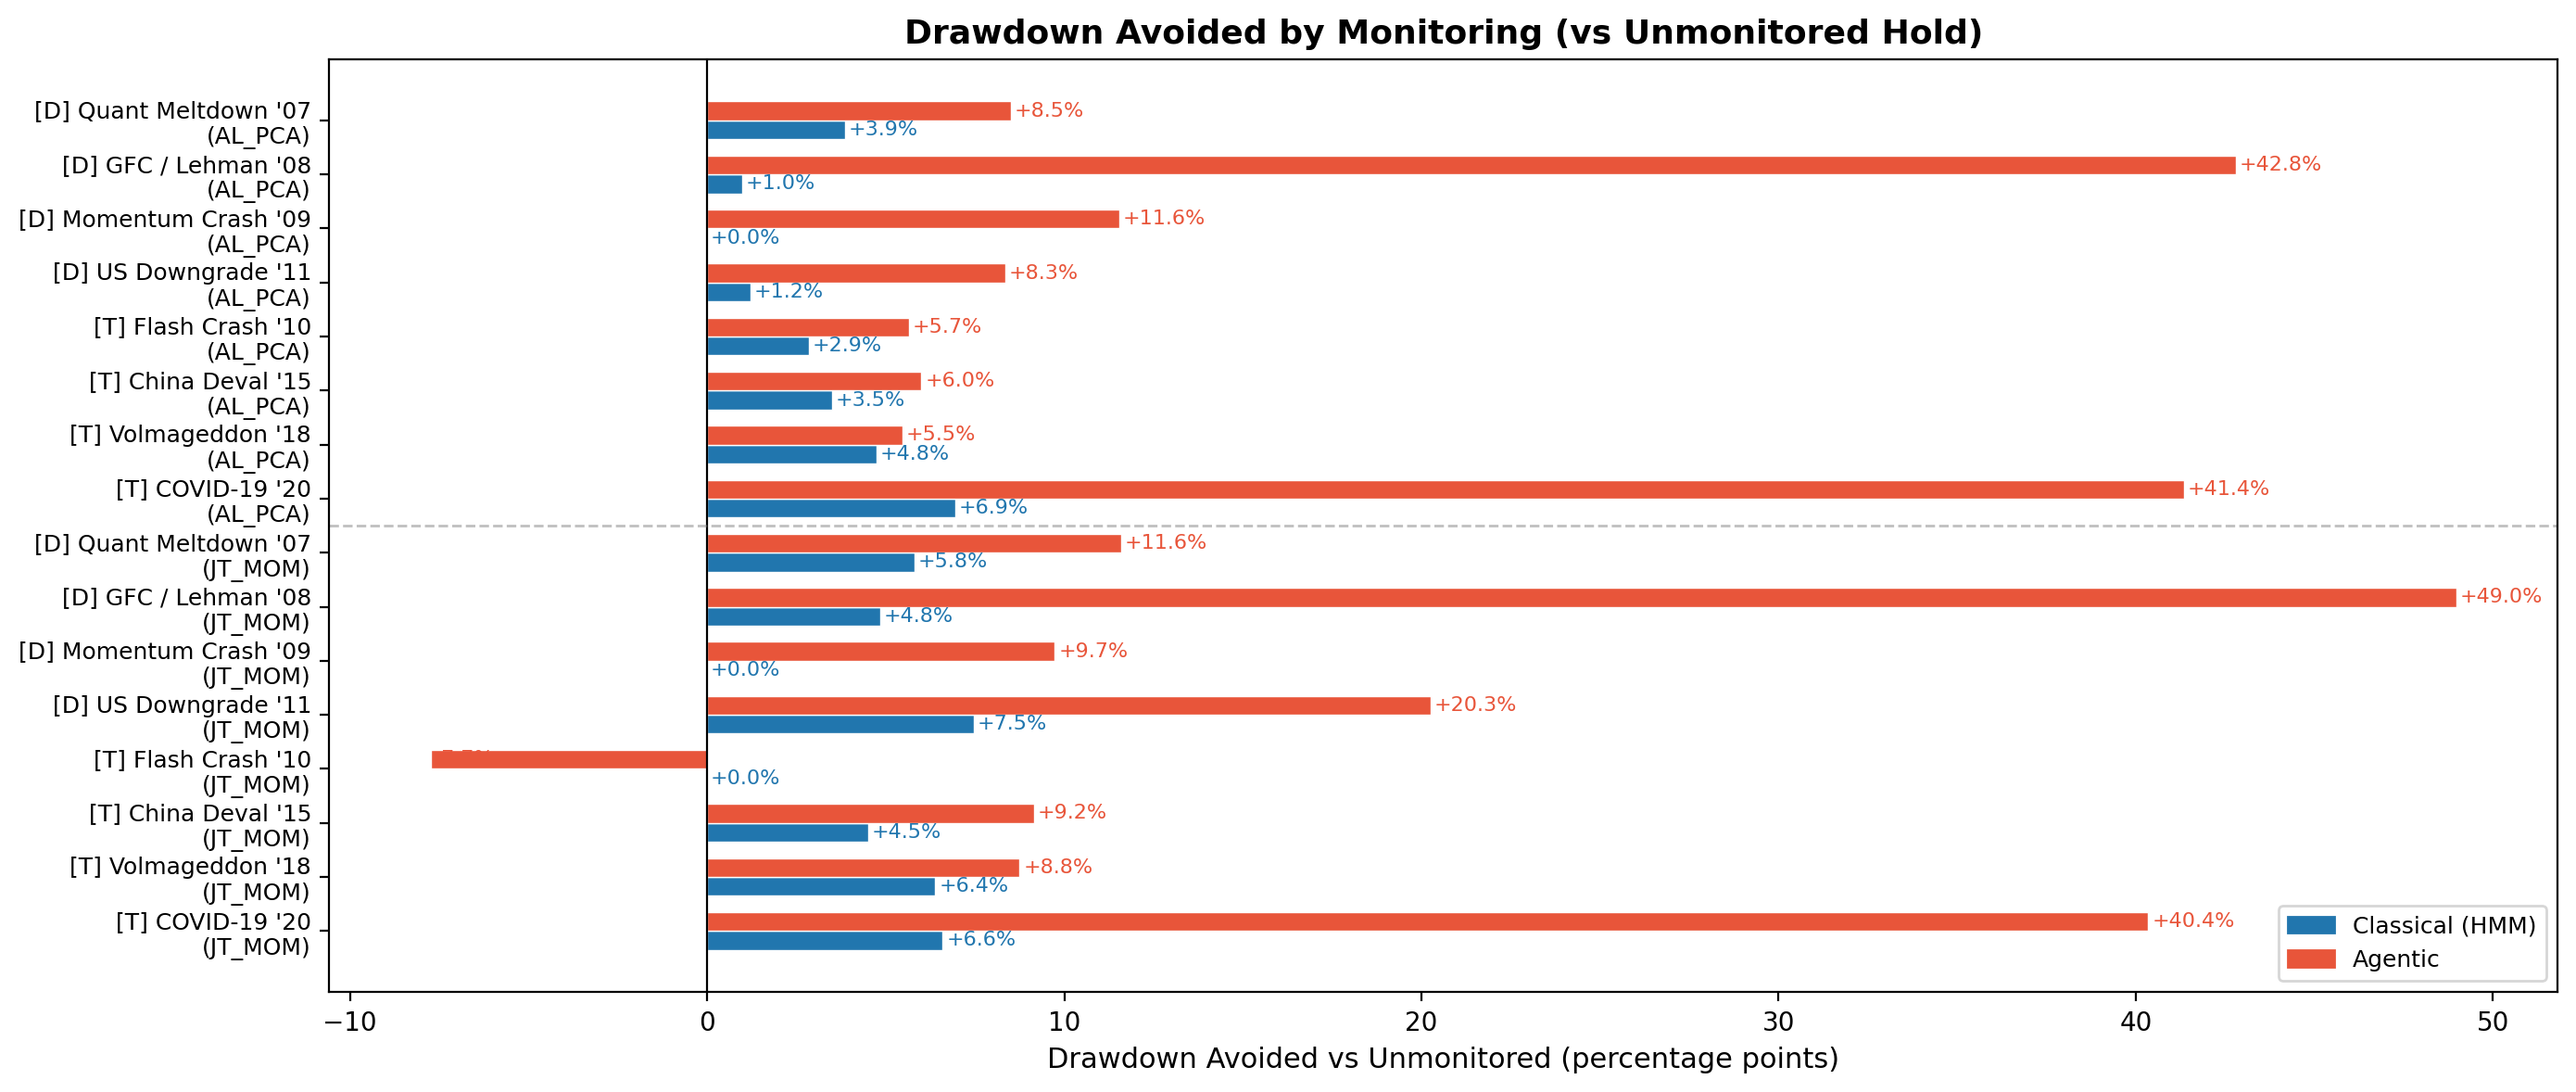
\includegraphics[width=0.8\textwidth]{monitoring/results/figures/fig11_drawdown_avoided.png}
\caption{Drawdown avoided (pp) per event window. The agentic arm avoids more
drawdown in 11 of 13 windows (one tie, one reversal).}
\label{fig:dd-avoided}
\end{figure}

\subsection{Robustness, Leakage, and Operations}\label{sec:results-ops}

\textbf{Onset sensitivity.} Re-scoring against curve-derived onsets yields
$-16.4$\,d ($p = 0.0039$) on the development set and $-11.8$\,d ($p = 0.0625$)
on the test set; rank ordering is unchanged. Using the aggregate rule instead
of the HMM as comparator widens the agentic advantage (aggregate detected 4/8
dev events vs.\ HMM's 6/8), so the HMM is the conservative baseline.

\textbf{Leakage bound.} On flash crash 2010 (AL\_PCA), Condition~A detected
with latency 5\,d, Condition~B (date-masked) with latency 0\,d, and
Condition~C recalled 10/10 synthetic windows. With
$\text{perf}_A = \text{perf}_B = \text{perf}_C = 1.0$, the memorisation bound
is $\leq 0$ and detection is classified \textbf{evidence-driven}. The B
$\approx$ A result directly manipulates the date channel; the high Condition~C
recall should be read cautiously since synthetic windows use an untrained HMM.

\textbf{Operational metrics.} Mean LLM calls per trading day are 1.09 (0.10 on
sparse-news calm 2004--2006 to 2.0 on quant meltdown 2007); wall-clock cost is
4.6\,s typical and 8.4\,s worst case per day, so a full window completes in
6--12 minutes, feasible for end-of-day monitoring. News-agent JSON failures on
non-skip days range from 0\% to 79\% (dense-news calm windows): failures
suppress alarms, so they bias \emph{against} the agentic arm for latency but
\emph{in favour} of it for FPR (Deviation~7); the latency advantage is
therefore conservative, the FPR comparison is not.

% ============================================================
\section{Discussion}\label{sec:discussion}

\textbf{Why earlier.} Two mechanisms drive the latency advantage. First, news
anticipation: coverage of developing crises precedes their statistical
manifestation in returns (quant-meltdown coverage of crowded quantitative
strategies appeared in late July 2007, enabling 0-day latency where the HMM
needed 7 days of anomalous returns). Second, multi-signal fusion: the
supervisor can escalate on the conjunction of individually sub-threshold
signals, whereas classical detectors observe returns alone. The advantage is
largest where the return stream never exhibits the volatility signature the
HMM is calibrated for (GFC 2008 and momentum crash 2009 on JT\_MOM).

\textbf{Why FPR is not better.} FinBERT stress saturates near 0.97 on
essentially every day with news (mean 0.971 on calm 2013--2014 and on GFC
2008 alike), so the 0.60 triage threshold degenerates into a ``does news exist
today?'' gate: dense-news days bypass skip mode, and the 1.5B supervisor lacks
the precision to separate concerning signals from routine financial noise,
over-escalating on calm windows.

\textbf{Power and the COVID-19 miss.} The 5-pair test set cannot reject after
Holm correction even in the best case (Section~\ref{sec:method-endpoints});
this follows from the AL\_PCA curve ending in 2014, not from the results. The
agentic arm's only test-set miss is COVID-19 2020. News was available (40
articles/day across all 82 days), but early pandemic coverage was dominated by
ambiguous general-volatility headlines; the classical HMM detected at 14\,d
from returns alone. A 1.5B model may lack the capacity to interpret an
unprecedented shock as a regime change from ambiguous text.\label{sec:power}

\textbf{Limitations.} (1)~Small samples: 8 development and 5 test pairs; the
confirmatory set cannot reach significance. (2)~Single model and single news
corpus; findings may not transfer. (3)~The FPR scoring asymmetry favours the
agentic arm, making the null FPR result conservative but not symmetric.
(4)~The PnL simulation is frictionless with no re-entry. (5)~Famous, heavily
documented test events carry memorisation risk; the leakage harness covers one
test window. (6)~US large-cap equities only. (7)~Fifteen protocol deviations,
mostly infrastructure, are disclosed in the repository; none alter prompts,
thresholds, or scoring post-freeze.

% ============================================================
\section{Conclusion}\label{sec:conclusion}

In this preregistered comparison, an LLM-based agentic monitor detected regime
breaks significantly earlier than classical change-point detection on the
development set ($-9.75$\,d, Holm $p = 0.0156$; recall 8/8 vs.\ 6/8), with a
directionally consistent but underpowered test set ($-4.4$\,d, $p = 0.25$).
The FPR co-primary endpoint did not favour the agentic arm, tracing to
saturation of the sentiment-based triage gate. Multi-signal fusion of returns,
news, and macro context thus shows genuine promise for earlier detection, with
exploratory economic value (8.28\,pp mean drawdown avoided per event), but
false-positive control requires redesigned triage (change-in-sentiment or
learned routing), larger models for supervisor precision, longer backtest
curves for confirmatory power, and leakage harness coverage of all test
windows.

% ============================================================
\section*{Data and Code Availability}

Code, prompts, result artifacts, and the full deviation log are available at
\url{https://github.com/PC1101/In-Market-Agentic-AI-Monitoring-Application-in-Financial-Market}
(tag \texttt{eval-freeze-v1} pins the evaluated code). The FNSPID corpus is
subject to its original license and must be obtained from the source; all
derived evaluation artifacts are included. Experiments used Ollama
(qwen2.5:1.5b) and ProsusAI/FinBERT on consumer hardware.

\section*{References}

\begin{description}[font=\normalfont, leftmargin=1.5em, labelindent=0em, itemsep=0pt]
\item Adams, R.~P. \& MacKay, D.~J.~C. (2007). Bayesian online changepoint
  detection. \emph{arXiv:0710.3742}.
\item Araci, D. (2019). FinBERT: Financial sentiment analysis with pre-trained
  language models. \emph{arXiv:1908.10063}.
\item Avellaneda, M. \& Lee, J.-H. (2010). Statistical arbitrage in the US
  equities market. \emph{Quantitative Finance}, 10(7), 761--782.
\item Daniel, K. \& Moskowitz, T.~J. (2016). Momentum crashes. \emph{Journal
  of Financial Economics}, 122(2), 221--247.
\item Dong, Z., Wang, Z., Li, X. \& Zhou, Y. (2024). FNSPID: A comprehensive
  financial news dataset. \emph{Proceedings of the AAAI Conference}.
\item Hamilton, J.~D. (1989). A new approach to the economic analysis of
  nonstationary time series. \emph{Econometrica}, 57(2), 357--384.
\item Holm, S. (1979). A simple sequentially rejective multiple test
  procedure. \emph{Scandinavian Journal of Statistics}, 6(2), 65--70.
\item Jegadeesh, N. \& Titman, S. (1993). Returns to buying winners and
  selling losers. \emph{Journal of Finance}, 48(1), 65--91.
\item Khandani, A.~E. \& Lo, A.~W. (2007). What happened to the quants in
  August 2007? \emph{Journal of Investment Management}, 5(4), 29--78.
\item Page, E.~S. (1954). Continuous inspection schemes. \emph{Biometrika},
  41(1/2), 100--115.
\end{description}

% ============================================================
\appendix

\section{Protocol Deviations}\label{app:deviations}

Table~\ref{tab:deviations} summarises all 15 deviations from the preregistered
protocol; full narratives with evidence and timestamps are maintained in the
repository (\texttt{docs/DEVIATIONS.md}).

\begin{table}[htbp]
\centering
\scriptsize
\setlength{\tabcolsep}{4pt}
\caption{Protocol deviations. ``Bias'' indicates whether the deviation favours
or disfavours the agentic arm for the affected endpoint.}
\label{tab:deviations}
\begin{tabular}{@{}p{0.5cm} p{3.1cm} p{3.3cm} p{4.2cm} p{3.2cm}@{}}
\toprule
\# & Preregistered & Actual & Rationale & Bias direction \\
\midrule
1 & llama3.2:3b & qwen2.5:1.5b & Failed JSON benchmarks (11/30 vs.\ 30/30);
    substituted before eval & Smaller model \\
2 & 90\% completeness & 80\% completeness & Include gfc\_2008 AL (84\%); all
    missing days post-detection & Includes 1 more pair \\
3 & AL\_PCA on china\_deval & Excluded & PIT curve ends 2014 & Fewer test pairs \\
4 & Triage skips calm days & 0\% skip on 2013--2014 & FinBERT saturation &
    Inflates FPR (against agentic) \\
5 & Supervisor-day completeness & Triage-day completeness & Triage = attempted;
    supervisor = succeeded & Includes gfc JT \\
6 & Stub latencies & Real-model latencies & Stub was provisional & None \\
7 & Not specified & News-agent failures documented & 0--79\% failure rate on
    non-skip days & Latency: against; FPR: for agentic \\
8 & Calibrated detector params & Default params & Calibrated grid computed but
    never wired in; HMM unaffected & Flatters agentic latency \\
9 & Symmetric FPR scoring & Asymmetric (cluster vs.\ alarm-day) & Analysis code
    difference & Favours agentic FPR \\
10 & Leakage on all test events & One test window covered & Harness incomplete
    at freeze & Partial coverage \\
11 & Single test-set pass & Rerun after runner death & Infrastructure outage,
    not result-shopping & None \\
12 & No resume logic & Day-level resume + recovery & Availability fix; identical
    prompts at $T = 0$ & Availability only \\
13 & Inline news queries & Two-pass context cache & VRAM contention on
    covid\_2020 & None (identical inputs) \\
14 & No per-day retry & 15\,s cooldown + ping + 1 retry & GPU thermal throttle &
    Availability only \\
15 & Full 40-article cap & 10 articles on 3 thermal-stall days & Prevent
    re-triggering stall & Conservative (less info) \\
\bottomrule
\end{tabular}
\end{table}

\section{Triage Hyperparameters}\label{app:triage}

\begin{table}[htbp]
\centering
\footnotesize
\caption{Triage hyperparameters (fixed a priori, preregistration \S6.2).}
\begin{tabular}{lrl}
\toprule
Parameter & Value & Purpose \\
\midrule
\texttt{STRESS\_CHEAP}    & 0.30 & FinBERT stress $\to$ cheap mode \\
\texttt{STRESS\_THINKING} & 0.60 & FinBERT stress $\to$ thinking mode \\
\texttt{HIT\_Z\_THINKING} & 2.0  & News intensity $z \to$ thinking mode \\
\texttt{RECENT\_DAYS}     & 3    & Detector lookback (calendar days) \\
\texttt{COVERAGE\_DAYS}   & 7    & News context window (calendar days) \\
\texttt{BASELINE\_PAD}    & 120  & $z$-score baseline history (calendar days) \\
Temperature               & 0.0  & Greedy decoding (deterministic) \\
Max articles              & 40   & Per-day article cap to news agent \\
\bottomrule
\end{tabular}
\end{table}

\end{document}
